\documentclass{standalone}
\usepackage[utf8]{inputenc}
\usepackage{fontspec}
\usepackage{tikz}
\usetikzlibrary{arrows.meta, positioning}

\setmainfont{Iosevka Nerd Font}

\begin{document}

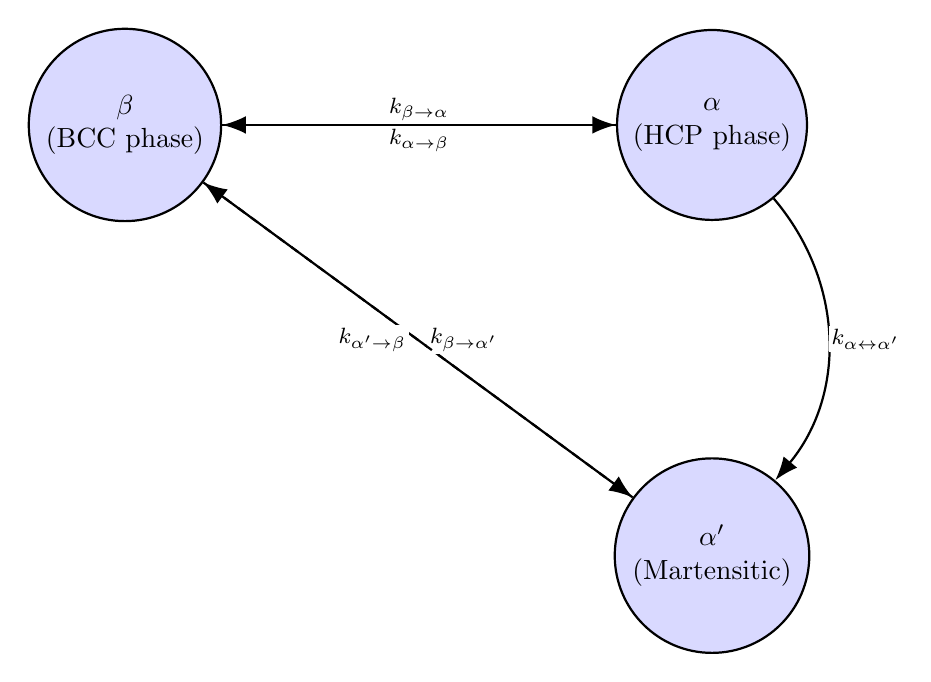
\begin{tikzpicture}[
    state/.style={circle, draw, thick, minimum size=2cm, align=center, fill=blue!15},
    arrow/.style={-{Latex[length=3mm]}, thick},
    eq/.style={midway, fill=white, font=\footnotesize, inner sep=1pt}
]

% Nodes: Ti64 phases
\node[state] (beta) {$\beta$ \\ (BCC phase)};
\node[state, right=5cm of beta] (alpha) {$\alpha$ \\ (HCP phase)};
\node[state, below=3cm of alpha] (alphaP) {$\alpha'$ \\ (Martensitic)};

% Arrows with kMC transition rates (symbolic)
\draw[arrow] (beta) -- node[eq, above] {$k_{\beta \to \alpha}$} (alpha);
\draw[arrow] (alpha) -- node[eq, below] {$k_{\alpha \to \beta}$} (beta);

\draw[arrow] (beta) -- node[eq, right, xshift=3pt] {$k_{\beta \to \alpha'}$} (alphaP);
\draw[arrow, dashed] (alphaP) -- node[eq, left, xshift=-3pt] {$k_{\alpha' \to \beta}$} (beta);

% Optional curved arrow between alpha and alpha'
\draw[arrow, bend left=40] (alpha) to node[eq, right] {$k_{\alpha \leftrightarrow \alpha'}$} (alphaP);

\end{tikzpicture}

\end{document}
